% !TEX root = ./robust.tex

\section{Introduction}
\label{sec:intro}

In this paper we study robust regression in the setting where the noise has outliers or contaminated values,
and the model parameters are estimated by minimizing the residual sum of absolute values. We adopt the standard regression model $y_i=x_i^T\beta^*+z_i$ for $n$ data points $(x_i,y_i)$, but assume that the noise is distributed according to a mixture, with $z_i\sim (1-\epsilon)P_i+\epsilon Q_i$ independently. The default noise distribution $P_i$ is assumed to have ``nice'' properties, but the corrupting distribution
$Q_i$ is completely arbitrary. The parameter $\epsilon$ indicates the fraction of the observations $y_i$ that are corrupted. The quantities $\epsilon$, $P_i$ and $Q_i$ are unknown; only the points $(x_1, y_1), \ldots, (x_n, y_n)$ are observed.


Figure 1 shows two examples that illustrate the robustness of median regression
in the case of a single predictor variable. Here the noise $P_i$ is heteroskedastic, and 75\% of the response values are corrupted. Nonetheless, the estimated slope is very close to the true parameter. We can gain some intuition for this by observing that since the corrupting noise is independent of the predictor variable, the outliers are ``parallel'' to the regression function. The focus of this paper is to understand this behavior quantitatively, to determine conditions and scaling regimes under which median regression is provably effective, in both low and high dimensions.

\begin{figure*}[t]
  \begin{tabular}{cc}
    \hskip-3pt
    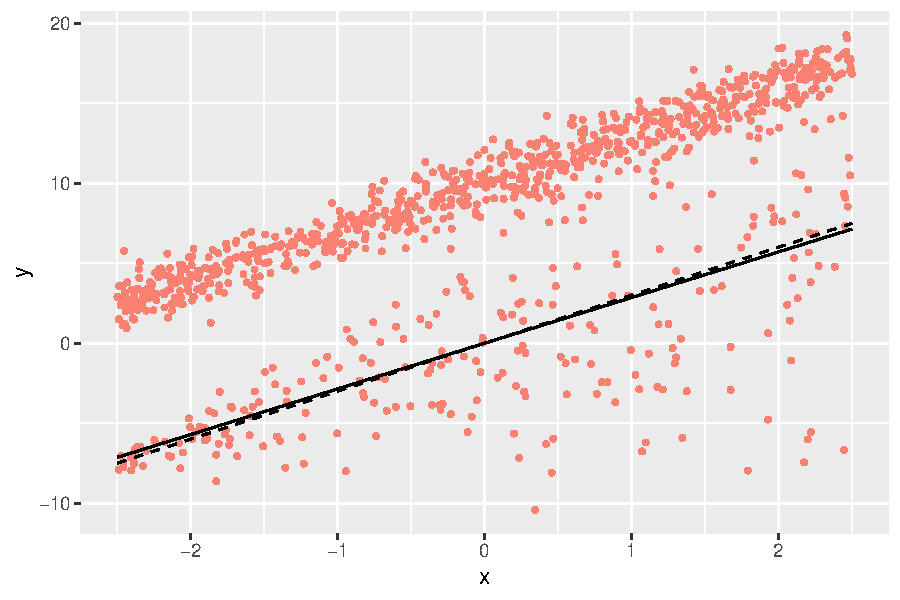
\includegraphics[width=.48\textwidth]{figures/fig1a} &
    \hskip-3pt
    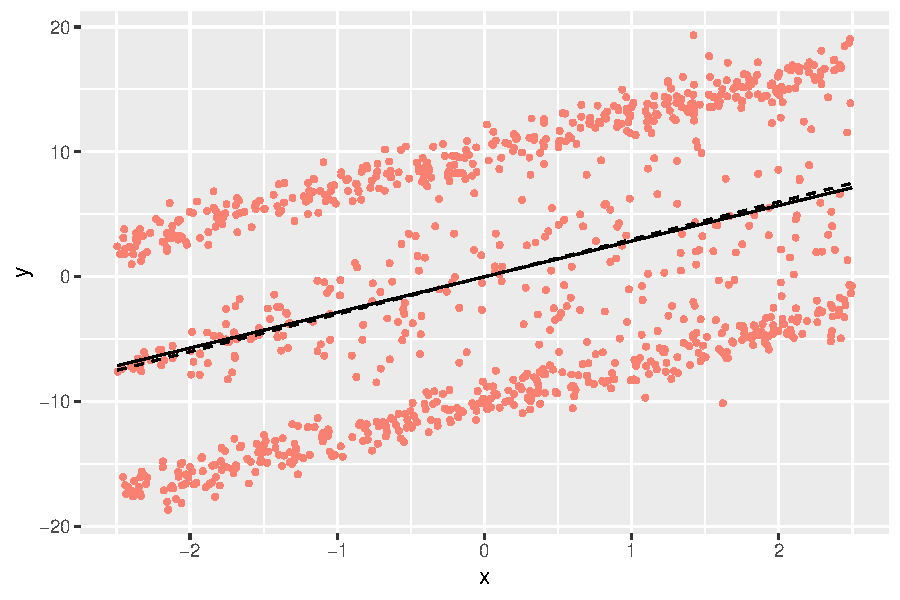
\includegraphics[width=.48\textwidth]{figures/fig1b}\\[-5pt]
  \end{tabular}
\caption{Median regression for corrupted data with $n=1{,}000$ and $\epsilon=0.75$.
The baseline noise is heteroskedastic, with distribution $P_i = N(0, (1.5 x_i + 4)^2)$
for data point $x_i$. Left: Corrupting distributions
$Q_i = N(10, 1)$. Right: Corrupting distributions $Q_i = N(10 \cdot W_i, 1)$ where $W_i$ are
independent Rademacher random variables. The solid line is the true regression
function, and the dashed line is the fit using median regression.}
\label{fig:exp}
\vskip20pt
  \begin{center}
    \begin{tabular}{cc}
      \hskip-10pt
      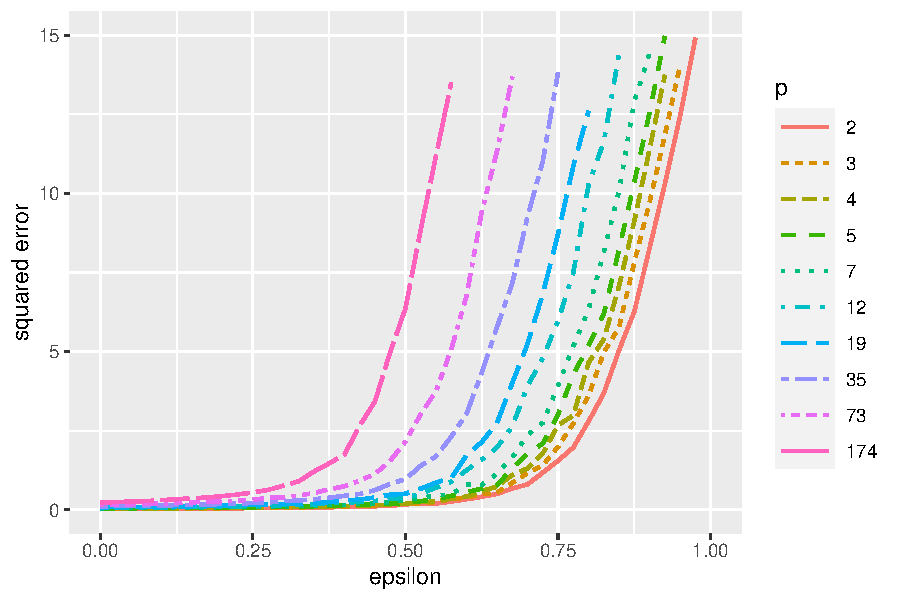
\includegraphics[width=.48\textwidth]{figures/fig2a}&
      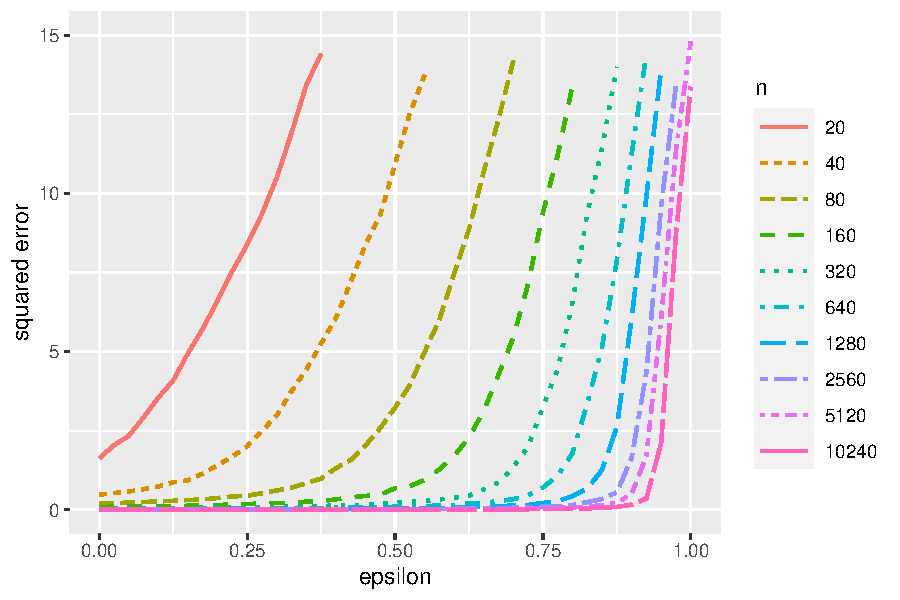
\includegraphics[width=.48\textwidth]{figures/fig2b}\\[-5pt]
    \end{tabular}
  \end{center}
\caption{Robust lasso for the linear model  $y=X\beta + z$ with design points $X_{ij}\sim N(0,1)$.
Left: Dimension $p$ varying as $p_{j} = e^{\rho^j}$, rounded down to the nearest integer, with $\rho=1.2$; the sample size is fixed at $n=100$, and $s=2$. Right: Dimension fixed at $p=10$ with $s=5$ relevant variables; the sample size $n$ is varied according to
$n_j = 2^j \cdot 20$ for $j=0,\ldots, 9$. The vertical axis shows the squared error $\|\hat \beta - \beta^*\|^2$ averaged over multiple trials.}
\end{figure*}

When the data are high dimensional, we add an $\ell_1$ penalty to the objective function, resulting in the estimator
\begin{equation}
  \wh{\beta}=\argmin_{\beta\in\mathbb{R}^p}\left[\frac{1}{n}\|y-X\beta\|_1+\lambda\|\beta\|_1\right].
  \label{robustlasso}
\end{equation}
This optimization is equivalent to a linear program, and can be thought of as a robust Lasso estimator. The main result in this paper implies that the error of this estimator scales as
\begin{equation}
  \|\hat \beta - \beta^*\|  = O_P\left(\frac{1}{1-\epsilon} \sqrt{\frac{s\log(p)}{n}}\right),
\end{equation}
under appropriate assumptions.
Here $s = \|\beta^*\|_0$ is the number of nonzero coefficients in the true model $\beta^*$, $n$ is the sample size, and $p$ is the number of predictor variables. The assumptions and precise statement of this result are given in Section~\ref{sec:main}. The primary aspect of this scaling that we highlight here is the factor of $1/(1-\epsilon)$, which implies that even for a large proportion $\epsilon \to 1$ of corrupted values, the model is consistently estimated by the robust lasso as the sample size increases. Figure~2 illustrates this scaling behavior with respect to $\epsilon, n, p$ in simulation.

In our analysis of the estimator \eqref{robustlasso}, it is seen that the optimal regularization parameter does not depend on the noise distributions $P_i$. In other words, the
estimator is pivotal with respect to the parameters of the noise, viewed as nuisance parameters.
In contrast, algorithms such as the lasso and iterative thresholding  require knowledge of the noise variance \citep{bickel2009simultaneous,suggala2019adaptive}.
The pivotal property is particularly important in the robust setting, where the
noise variance is not identifiable; we discuss this point further in Section~\ref{sec:main}.
In addition, we show how the robust lasso can be effective when the design variables $X_j$ and the noise distributions $P_i$ have heavy tails.
In fact, this procedure is robust to arbitrary contamination, heavy-tailed noise, and heavy-tailed design distributions simultaneously. Algorithmically, we show how the linear program \eqref{robustlasso} can be reformulated as median regression with respect to a transformed design matrix.

In the following section we review the existing literature on the problem of robust regression for corrupted noise, which has seen significant attention in recent years. We also relate this problem to previous work that considers corrupted design and noise together. The main results of the paper are presented in Section~\ref{sec:main}, where we establish the scaling behavior of median regression under different assumptions. We separate the cases where the design variables are assumed to have sub-Gaussian and heavy tails. A series of simulations that exhibit close correspondence with this theory are presented in Section~\ref{sec:experiments}. The detailed proofs of these results are collected in Section~\ref{sec:proofs}.  Finally, we discuss these results and their implications for applications in Section~\ref{sec:discuss}. We also mention directions for future research, including extensions to robust quantile regression.

% WLOG assumption on median zero
